\chapter{Theory {\color{red} Would call this Section Method}}%
\label{ch:theory}

In this chapter we introduce the theoretical idea of our Bayesian modeling of source separation. First we explicitly state our chosen model of the problem, next derive a suitable optimization objective from it and then explain how we can optimize towards that.

We propose the graphical model as shown in \cref{fig:graphical_model} as the generative story of the source separated music tracks. For each source a sample is taken from the latent source distribution. The observed mix is generated deterministically from the full set of sources. Without loss of generality we fix this function to be the mean.

\begin{marginfigure}[-15em]
    \begin{tikzpicture}
    \node[obs]                (x) {\(\x\)};
    \node[latent, left=of x]  (z) {\(\z\)};

    \edge {z} {x} ; %

    \plate {xz} {(x)(z)} {\(N\)} ;
\end{tikzpicture}
%
    \caption{The used graphical model for the source separation task. We have the latent source channel variables \(\s_k\). Exemplary here, as in our data, we have four sources. The mix \(\m\) is observed.}%
    \label{fig:graphical_model}
\end{marginfigure}

Our stated task in \sref{sec:question} is to model the density \(p(\s_k|\m)\) without using sample tuples \((\m, \{\s_1,\…,\s_N\})\). We follow the same steps as previously shown for the latent variable models. First we introduce a approximate posterior \(\aprxpost\) for each source channel. Next we express the mix density as the expectation over those posteriors:

\begin{align}
    \log p(\m)
    &= \E_\aprxpost^N \left[ \log p(\m) \right]\label{eq:expectation_over_approx_post}
\end{align}

From here derive the ELBO in the same way as before, just now with \(N\) priors instead of one:

\begin{fullwidth}
    \newcommand{\post}{p(\s_1,\…,\s_N|\m)}
    \begin{align}
        \E_\aprxpost^N \left[ \log p(\m) \right]
        &= \E_\aprxpost^N \left[ \log \÷{p(\m,\s_1,\…,\s_N)}{\post} \right]\\
        &= \E_\aprxpost^N \left[ \log \÷{p(\m|\s_1,\…,\s_N) \· \Π_k^N p(\s_k)}{\Π_k^N \aprxpost} + \log \÷{\Π_k^N \aprxpost}{\post} \right]\\
        &\geq \Σ_k^N \E_\aprxpost \left[ \log \÷{p(\s_k)}{\aprxpost} \right]
             +\E_\aprxpost \left[ p(\m|\s_1,\…,\s_N) \right]\label{eq:final_elbo}\\
    \end{align}
\end{fullwidth}

Like in the VAE we now formulate the lower bound for approximting the graphical model with the approximate posterios \(\aprxpost\) which we will parametrize with deep neural networks. The source priors are estimated \I{a-priori} and  independtly and are also parametrized by neural networks. Here we introduce a fairly big assumption, namely that we can model the source distributions independtly from each other when modeling the joint:

\begin{align}
    p(\m,\s_1,\…,\s_N) &\equiv p(\m|\s_1,\…,\s_N) \· \Π_k^N p(\s_k)
\end{align}

It is intuitive that this assumption does not, in general, hold for the musical domain. We can expect a different behaviour for a guitar in a song involving a second source like a percussion set. The joint of those two models is different than their independent densities. Nevertheless this assumption is crucial to be able to model the prior instrumental models without needing the tuples \((\s_1,\…,\s_N)\) of co-occurring stems.

Finally we note that this assumption is not being used for the independent approximate posteriors. While the true posterior certainly is the posterior of the joint source model, we choose our approximate posteriors to be independent. The expectation in \eqref{eq:expectation_over_approx_post} over those is still correct. The error arising from the independence assumption is captured in the thightness of the ELBO. {\color{red} I would add a paragraph that states what choices need to be made: Encoder, Decoder, Prior}

\section{Modeling the priors}
The first step in the training procedure is the training of the independent source priors \(p(\s_k)\). We have to choose a model for estimating the density that results in smooth, tight densities but also is capable enough to capture the complex data space of audio data. We choose to estimate the priors with flow models for which we gave an overview in \cref{methods}. For different representation of the input different network architectures are mode suited. We experiment both with inputing directly the time-domain wave but also modeling on top of a spectral transformation of the time-domain data.

The two main variants of normalizing flows we build our priors from are the RealNVP and Glow. Their most important difference is the different formulation of the coupling layers. For the coupling layers we have to split the layer input into two equally sized subsets, one of whom will be transformed using an invertable transformation parametrized by the other. The RealNVP masks the data spatially or over the channels in two different groups. Glow learns a \(1\× 1\)-convolution which permutes the data channel-wise and than just splits the data along the channel dimension into two. For both RealNVP and Glow prior works exists adapting the architecture specifically to the time-series domain by integrating WaveNet modules, FloWaveNet~\cite{kimFloWaveNet2019a} and WaveGlow~\cite{prengerWaveGlow2018}, respectively. \todo{wat about waveflow}

For the case of the time-domain representation, the data has only one channel (mono-audio). Therefore a Glow-like shuffleing of channels is not possible and we resort to using spatial masking for the coupling layers. In the case of using a spectral representation of the audio data we can also experiment with channel-shuffleing.

\itodo{blabla}

\subsection{Fixing the priors}

\itodo{blabla}

\section{Modeling the posteriors}

Assuming we have now a set of meaningful, discriminative priors \(p(\s_i)\) we need to combine the independent models to extract sources \(\{\s_i\}\) given a mix \(\m\). At the beginning of this section we already introduced the imagined generative model and derived the lower bound for the approximate posterior. Taking a step back again and looking at the posterior we have two general possibilities to retrieve samples from the posterior \(p(\s_i | \m)\).

\begin{align}
    p(\s_i|m)
    &= \÷{p(\m|\s_i)\· p(\s_i)}{p(\m)}
\end{align}

First we can model the approximate posterior \(\aprxpost\). By doing so we train a new subsequent function which directly retrieves the predicted sources given a mix. This method is, in principle, the same as we would see in a normal variational-autoencoder. Alternatively, finding the actual posterior to difficult to model, we can sample \(\s_i \sim p(\·|m)\) without computing the actual distribution.

\subsection{Variational-autoencoder}

\itodo{blabla}

\subsection{Langevin Dynamics}
The second option for estimating the posterior \(p(\s_i | \m)\) is iteratively sampling from the prior, under the the mixing constraint, using Langevin dynamics~\cite{nealMCMC2012}. While they are a classical approach to stochastic modeling of a dynamical modelcular system, \textcite{wellingBayesian2011} has shown how to employ Langevin dynamics as an MCMC sampling process to estimate the posterior in Bayesian modeling. With Stochastic Gradient Langevin Dynamics (SGLD) we can sample from \(\s_i \sim p(\· | \m)\) without computing, explicitly, the posterior \(p(\s_i | \m)\).

\itodo{explanation}

The idea of using SGLD in combination with deep parametrized priors was, concurrently to this work, introduced in \textcite{jayaramSource2020}. The authors argue that direct optimization under the prior distribution is not successfull due to the severe peakedness of the priors. Thus, they argue, the stochasticity, added with the Gaussian noise in SGLD, is needed to not get stuck in local optimas under the manifold. We challenge that explanation as it is, blabla

\begin{figure}[]
    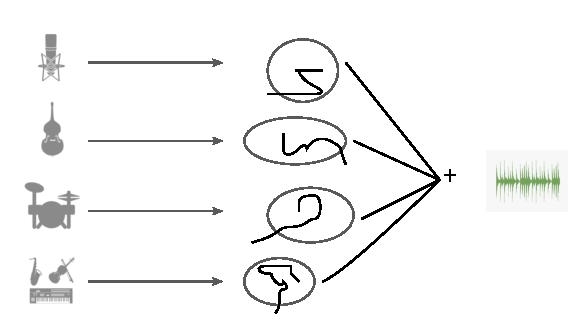
\includegraphics{sampling.eps}
    \caption{The method visualized}
    \label{fig:method}
\end{figure}

{\color{red} I like the section so far, but I think you should emphasize more what are the challenges, e.g., for both the VAE approach and the Langevin dynamics we need a prior and a posterior. In addition, since we have a probabilistic approach we need to choose distributions for everything.}